\section{Présentation du projet}
Le projet que nous avons réalisé est un accordeur de guitare. Celui-ci a été codé à l'aide du logiciel utilisé lors des TPs, Matlab. Nous avons choisi d'implémenter une interface graphique, plus intuitive à utiliser. Celle-ci propose d'accorder sa guitare selon plusieurs accords fréquemment utilisés. La figure~\ref{interface} montre l'interface utilisateur de l'accordeur.

\begin{figure}[H]
\centering
\begin{subfigure}[b]{7cm}
	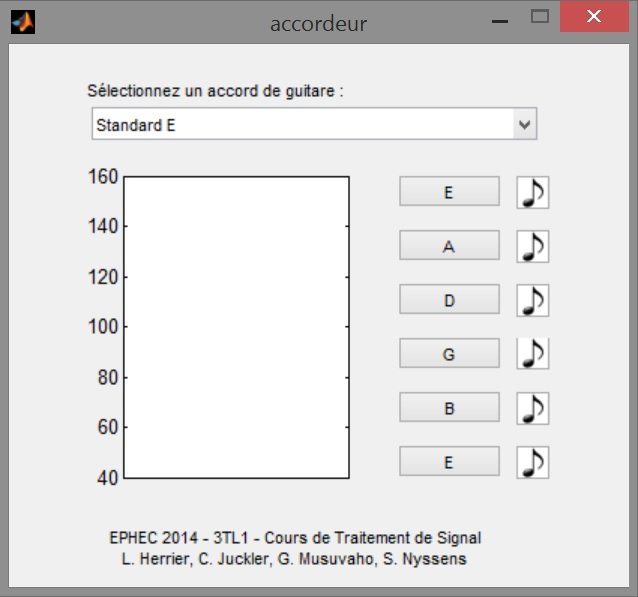
\includegraphics[width=6cm]{accordeur.jpg}
	\caption{Accordeur au démarrage}
\end{subfigure}
\begin{subfigure}[b]{7cm}
	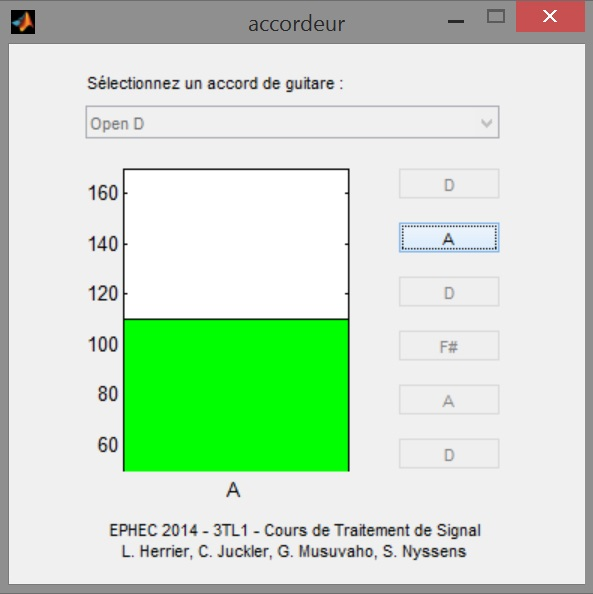
\includegraphics[width=6cm]{accordeurOn.jpg}
	\caption{Accordeur en train d'accorder}
\end{subfigure}
\caption{Interface utilisateur}
\label{interface}
\end{figure}

On peut voir sur les images ci-dessus la manière dont nous avons composé notre accordeur. Dans le haut de la fenêtre se trouve le menu de sélection des accords. Nous proposons divers accords fréquents pour la guitare : 
\begin{itemize}
\item L'accordage classique en\textit{ E}
\item Le \textit{Drop D}
\item L'\textit{Open D}
\item L'\textit{Open G}
\item L'accordage en \textit{quartes}
\end{itemize}
Les boutons de droite représentent les notes composant l'accord, ainsi que la possibilité d'écouter la note. Celui du dessus correspond à la corde du dessus lorsqu'on tient une guitare, autrement dit la note la plus grave. Enfin, le grand rectangle à gauche sert à visualiser si la corde de la guitare sélectionnée est bien accordée ou non. Le code couleur utilisé est classique : vert si la corde est correctement accordée, à 2Hz près, jaune-orange si la corde est trop haute ou trop basse à 15Hz près, et rouge si elle est hors des limites précédentes.\\

Lorsqu'une note est sélectionnée pour être accordée, un timer de 5 secondes s'enclenche. Il est possible pendant ce temps de jouer la corde pour l'accorder. De plus, les autres notes sont bloquées, ainsi que la sélection des accords, afin d'éviter les conflits.
